% =====================================================================
% OPENER: A Frugal Open-World NER Pipeline for the Legal Domain
% Target venue: NLLP @ EMNLP (ACL style). Double-blind submission.
% Switch "review" -> "final" for camera-ready, "preprint" for a named arXiv version.
% Compilation: pdflatex main && bibtex main && pdflatex main && pdflatex main
% =====================================================================
\documentclass[11pt]{article}

\usepackage[final]{acl}   % camera-ready : plus de ruler ni de numeros de page
% acl.sty forces \flushbottom, which stretches the glue between the result
% tables to equalise column heights and opens large gaps. Columns may end
% short instead: margins, fonts and spacing are untouched.
\raggedbottom
% acl.sty loads hyperref and colours every link darkblue, which is loud in the
% bibliography. Links stay clickable, they just render in the body text colour.
\hypersetup{colorlinks=true, citecolor=black, linkcolor=black, urlcolor=black}

% Standard ACL includes
\usepackage{times}
\usepackage{latexsym}
\usepackage[T1]{fontenc}
\usepackage[utf8]{inputenc}
\usepackage{microtype}
\usepackage{inconsolata}
\usepackage{graphicx}
\graphicspath{{assets/}{../assets/}}

% Project-specific packages used by the section files
\usepackage{amsmath,amssymb,amsfonts}
\usepackage{dsfont}       % \mathds{1} : indicator symbol (amssymb has no blackboard digit)
\usepackage{booktabs}
\usepackage{array}
\usepackage{float}        % [H] float placement
% The architecture figure spans both columns at full width: without this, LaTeX
% refuses to put a float that tall at the top of a page and defers it to the end.
\renewcommand{\topfraction}{0.92}
\renewcommand{\textfraction}{0.06}
\renewcommand{\floatpagefraction}{0.80}
\renewcommand{\dbltopfraction}{0.95}      % two-column floats use the dbl* limits
\renewcommand{\dblfloatpagefraction}{0.70}
\setcounter{dbltopnumber}{2}
% Tighter space around floats (document-level spacing only, margins untouched).
\setlength{\textfloatsep}{8pt plus 2pt minus 2pt}
\setlength{\intextsep}{8pt plus 2pt minus 2pt}
\setlength{\dbltextfloatsep}{8pt plus 2pt minus 2pt}
\usepackage{xcolor}
\usepackage{colortbl}
\usepackage{threeparttable} % short caption + notes block below each table (KBS-style)
\usepackage{pgfplots}
\pgfplotsset{compat=1.18}
\definecolor{hlyellow}{rgb}{1,0.93,0.5}   % OPENER-ZS rows
\definecolor{hlred}{HTML}{FECACA}         % OPENER-Sup rows

% --- Camera-ready (NLLP 2026) : marquage des revisions ------------------
% Tout ce qui a ete ajoute ou reecrit en reponse aux reviewers est enveloppe
% dans \rev{...}. Pour produire le PDF A SOUMETTRE, remplacer la definition
% par \newcommand{\rev}[1]{#1} : le texte redevient noir, rien d'autre ne
% bouge. Le PDF final ne doit PAS partir en rouge (regle ACL sur la couleur).
\newcommand{\rev}[1]{\textcolor{red}{#1}}
%\newcommand{\rev}[1]{#1}   % <-- decommenter pour la version finale

% --- figure palette (matches the general-domain OPENER paper, for consistent styling) ---
\definecolor{figamber}{HTML}{F59E0B}
\definecolor{figcyan}{HTML}{06B6D4}
\definecolor{figsky}{HTML}{0EA5E9}
\definecolor{figviolet}{HTML}{8B5CF6}
\definecolor{figgold}{HTML}{EAB308}
\definecolor{figgreen}{HTML}{10B981}
\definecolor{figpink}{HTML}{EC4899}
\definecolor{figred}{HTML}{DC2626}

% Zero-shot shorthand reused from the main paper
\newcommand{\zstr}{\textsc{OPENER-ZS}}
% Indicator function (dsfont renders the digit 1, unlike amssymb's \mathbb)
\newcommand{\indic}{\mathds{1}}

% \autoref names: ACL style capitalises cross-references as "Section"/"Appendix".
\renewcommand{\sectionautorefname}{Section}
\renewcommand{\subsectionautorefname}{Section}
\renewcommand{\subsubsectionautorefname}{Section}

\title{OPENER: A Frugal Open-World NER Pipeline for the Legal Domain}

% TODO CAMERA-READY : remplacer par les vrais auteurs et affiliations.
% Regles ACL : prenoms complets (pas d'initiales), pas de NOM en capitales,
% pas de footnote pour l'affiliation, et l'ordre/orthographe doivent coincider
% avec ce qui est saisi dans OpenReview.
\author{
  \rev{Thibault Garel} \\
  \rev{LyRIDS, ECE Paris} \\
  \rev{\texttt{garel.thibault14@gmail.com}} \\
}

\begin{document}
\maketitle

\begin{abstract}
Legal text is hard for named entity recognition. New statutes, parties and courts appear continually, and expert annotation is costly. Open-world NER assigns types that were not fixed at training time. These systems are built on general-domain text, though, and legal uses adapt them corpus by corpus and language by language. \rev{We take the opposite route, and apply OPENER unchanged}, a frugal pipeline of ready-to-use components. Its entity embedder is deliberately left generic, so its space is never fitted to one legal schema. We evaluate a zero-shot head (OPENER-ZS) and a supervised linear probe (OPENER-Sup) on four legal corpora, in English, Portuguese and German. The baselines are GLiNER, GNER, OWNER and a 4-bit Qwen, and we report quality (Adjusted Mutual Information), latency and energy jointly, over three seeds. The design holds under an English domain shift, and degrades cross-lingually. OPENER-ZS stays usable in English (up to 49.1 gold AMI), but it does not lead, and it weakens across languages (23.8 to 37.4). OPENER-Sup is barely affected (61.4 on average), and posts the best end-to-end score (35.9). Every system is then capped by the English detectors' recall, as low as 10.2\% on German. Both heads reach that ceiling at one to two orders of magnitude less latency and energy than the generative baselines. \rev{On detected mentions, the supervised head types 78.7\% correctly, against the detector's 64.6\%. A typing oracle over those same spans caps end-to-end quality at 70 AMI, the rest being mentions the detector never proposes.} Where labels exist, the supervised head is the practical operating point. Detection, not typing, is where adaptation should go first.

\end{abstract}

\section{Introduction}
\label{sec:introduction}

Named Entity Recognition (NER) extracts entities such as persons, organisations and dates from raw text. It is a foundational step in most information extraction pipelines. Standard NER systems are closed-set. They are trained once on a fixed inventory of types, and can only ever predict those types. Real-world applications rarely afford such a static inventory, and legal text is an extreme case. Entity inventories there are open and shifting, with new statutes, case citations, parties, courts, contractual instruments and jurisdictions. Documents are long and formulaic, annotation requires expert effort, and extraction errors carry material consequences. Re-annotating and retraining a tagger for every new type or sub-domain is rarely practical.

\emph{Open-world} NER targets precisely this regime. It recognises and types entities whose categories were not fixed at training time. Notable systems reach it by different routes. They score spans against type names \citep{zaratiana2024gliner}, tag generatively \citep{ding2024gner}, cluster a dedicated entity encoder into dynamically named types \citep{genest2025owner}, or prompt instruction-tuned models at far higher inference compute \citep{zhou2024universalner}. All of them are trained and evaluated on general-domain text. Their legal uses then adapt them per corpus, schema and language, either by fine-tuning a tagger or by prompting a large model anew. Few legal deployments can pay that price for every schema, sub-domain and jurisdiction. We take the opposite route, with one open-world pipeline whose components are never fitted to a legal corpus. We measure it component by component, to locate the bottleneck and show where the next annotation or compute budget should go.

We do this with OPENER \rev{(Open Partitioning Embedding for Named Entity Recognition)}, a frugal open-world pipeline \rev{assembled from} ready-to-use pretrained components. A frozen open-world detector proposes spans. A light contrastively fine-tuned, Matryoshka-truncatable embedder then represents them. That embedder is fine-tuned on general-domain entity spans, and never on a legal schema. This is a design choice rather than a shortcut. An open-world space must stay unspecialised, or it collapses into the closed-set taggers we are trying to avoid. The pipeline also runs one to two orders of magnitude cheaper in latency and energy than trained-encoder and generative baselines. Legal practice is rarely GPU-rich, and needs exactly that. We evaluate its two operating points. OPENER-ZS is a label-free head, built on label-name prototypes, transductive refinement and detector fusion. OPENER-Sup is a balanced linear probe, fit on the legal target labels. Our contributions are:
\begin{itemize}
\item \textbf{A frugal pipeline for legal NER.} We assemble an open-world pipeline from pretrained components, with \emph{no} legal-domain training of any of them, and we test both of its typing heads.
\item \textbf{A legal open-world benchmark.} Four legal NER corpora in three languages, English (SEC/EDGAR filings and Indian court judgements), Portuguese and German (Brazilian and federal court decisions). Eight systems are compared end to end under one protocol, both OPENER heads, the standard open-world baselines (GLiNER-S/M/L, GNER-T5 and OWNER), and a 4-bit Qwen2.5-1.5B.
\item \textbf{A three-axis, seed-averaged protocol.} We report quality (AMI), latency and energy jointly rather than accuracy alone, and average every OPENER score over three embedder-retraining seeds.
\item \textbf{An explanation of why the two heads diverge, and of where quality is lost.} OPENER-ZS stays usable on English legal text (up to 49.1 gold AMI), but it does not lead the zero-shot field. It trails GLiNER-M/L and, on average, OWNER. OPENER-Sup is barely dented by the domain shift ($61.4$ mean gold AMI), and posts the best end-to-end score (35.9). Its balanced probe draws boundaries between closely related legal types that a single label-name match cannot. \rev{Splitting each end-to-end score into detection and typing shows the probe typing $78.7\%$ of detected mentions correctly, against the detector's own $64.6\%$. Even a head typing all of them correctly would stop at ${\approx}70$ AMI rather than $100$. Mentions the detector never proposes cannot be recovered downstream.} Both heads are then capped by the English detectors' recall, down to $18.7\%$ on German for GLiNER-L and $10.2\%$ for GLiNER-M. In-language \emph{detection}, not typing, is therefore the first place further adaptation should go.
\end{itemize}

\section{Related Work}
\label{sec:related}

\subsection{Open-world and zero-shot NER}
The three open-world systems we compare against differ in backbone as much as in approach. GLiNER \citep{zaratiana2024gliner} scores spans against candidate type names with a DeBERTaV3 encoder \citep{he2023debertav3}. GNER \citep{ding2024gner} generates them with a sequence-to-sequence model \citep{raffel2020t5}. OWNER \citep{genest2025owner} trains a dedicated entity encoder, then clusters mentions into dynamically named types. Typing from type descriptions \citep{aly2021zeroshot} needs no labelled example at all. A complementary line distils or prompts billion-parameter language models for open NER, as in UniversalNER \citep{zhou2024universalner}, GoLLIE \citep{sainz2024gollie} and ChatIE \citep{wei2024chatie}. Our comparison also probes that compute and energy cost, \rev{through an instruction-tuned LLM baseline (Qwen2.5-1.5B in $4$-bit) sized to the hardware this paper measures everything on}. OPENER differs from all of these by reusing a pretrained embedding rather than training an encoder, which is what keeps it cheap enough for the legal setting we target.

\subsection{Legal NLP and legal NER}
Legal NLP is an active field, spanning summarisation, judgement prediction, question answering and information extraction, as a recent legal-NLP survey documents \citep{ariai2025legalnlp}. It is driven by the specialised vocabulary, the long formulaic documents and the jurisdiction-specific entity inventories of legal text. On the modelling side, domain-adapted language models such as LEGAL-BERT \citep{chalkidis2020legalbert} and multi-task benchmarks such as LexGLUE \citep{chalkidis2022lexglue} show that in-domain pretraining and evaluation matter for legal NLU.

The dominant approach to legal NER is to train or adapt a supervised tagger for each corpus, schema and language. LegNER \citep{karamitsos2025legner} domain-adapts BERT with span supervision for English legal NER and anonymisation. A Serbian legal NER study \citep{kalusev2025serbian} fine-tunes a BERT-type model for court rulings and releases a new dataset. The LegalEval shared task (SemEval-2023 Task~6) spurred systems such as a Bi-LSTM with Flair embeddings for Indian court judgements \citep{ramesh2023flairnlp}. Even LLM-based studies remain schema-bound. A financial NER study \citep{lu2025financial} prompts GPT-4o, LLaMA-3.1 and Gemini-1.5, and reports systematic failure modes on domain entities. These systems achieve strong in-corpus scores, but each one requires labelled data and (re)training tied to one schema and one language. E-NER \citep{au2022ener} annotates U.S.\ SEC/EDGAR filings with seven classes, including court, government body and legislation/act. \rev{Indian-Legal \citep{kalamkar2022indianlegal} tags Indian judgements with $14$ types, from judge and lawyer to precedent.} LeNER-Br \citep{luzdearaujo2018lenerbr} covers Brazilian court decisions with dedicated \emph{legislation} and \emph{case-law} tags. German-LER \citep{leitner2020germanler} annotates German federal decisions with a fine-grained 19-class schema.

Crucially, the E-NER study \citep{au2022ener} reports that NER models trained on general English degrade sharply on legal text, \rev{from $90.5$ F1 in-domain down to $61.1$ once tested on legal filings}. That is precisely the distribution shift we study. Rather than retraining a legal-specific tagger per corpus and language, we build a single open-world pipeline that no legal schema ever touches, and we measure how far it goes on all four of them (\autoref{sec:experiments}).

\subsection{Energy-aware evaluation}
Reporting efficiency alongside accuracy is increasingly advocated, from the Green AI agenda \citep{schwartz2020greenai} to energy audits of NLP training \citep{strubell2019energy}, systematic carbon reporting \citep{henderson2020systematic,patterson2022carbon} and whole-lifecycle views of AI's footprint \citep{wu2022sustainable}. At inference time specifically, a deployment-cost study \citep{luccioni2024power} finds general-purpose generative models orders of magnitude more expensive per query than task-specific ones. That is precisely the gap this frugal pipeline targets. We adopt the same three-axis view, on quality, latency and energy, measured with CodeCarbon \citep{codecarbon2024} and reported in the energy-times-grid-intensity accounting of \citet{lacoste2019quantifying}.

\section{Method}
\label{sec:method}

OPENER is built for the legal domain, yet none of its components is fitted to it. The detector and the entity embedder are ready-to-use checkpoints kept frozen, so no gradient step is ever taken on legal text. Only the typing head touches the legal side: OPENER-ZS consumes no legal label at all, deriving its prototypes from the type names and refining them on the unlabelled test mentions, while OPENER-Sup fits a linear classifier on the frozen embeddings of the target's training mentions, consuming legal labels without updating a single encoder weight. We therefore measure how far a frugal open-world pipeline goes on legal NER \emph{without} being retrained on it, which is the regime a legal deployment actually faces.

\begin{figure*}[t]
\centering
\IfFileExists{assets/opener-architecture-v3.pdf}{%
  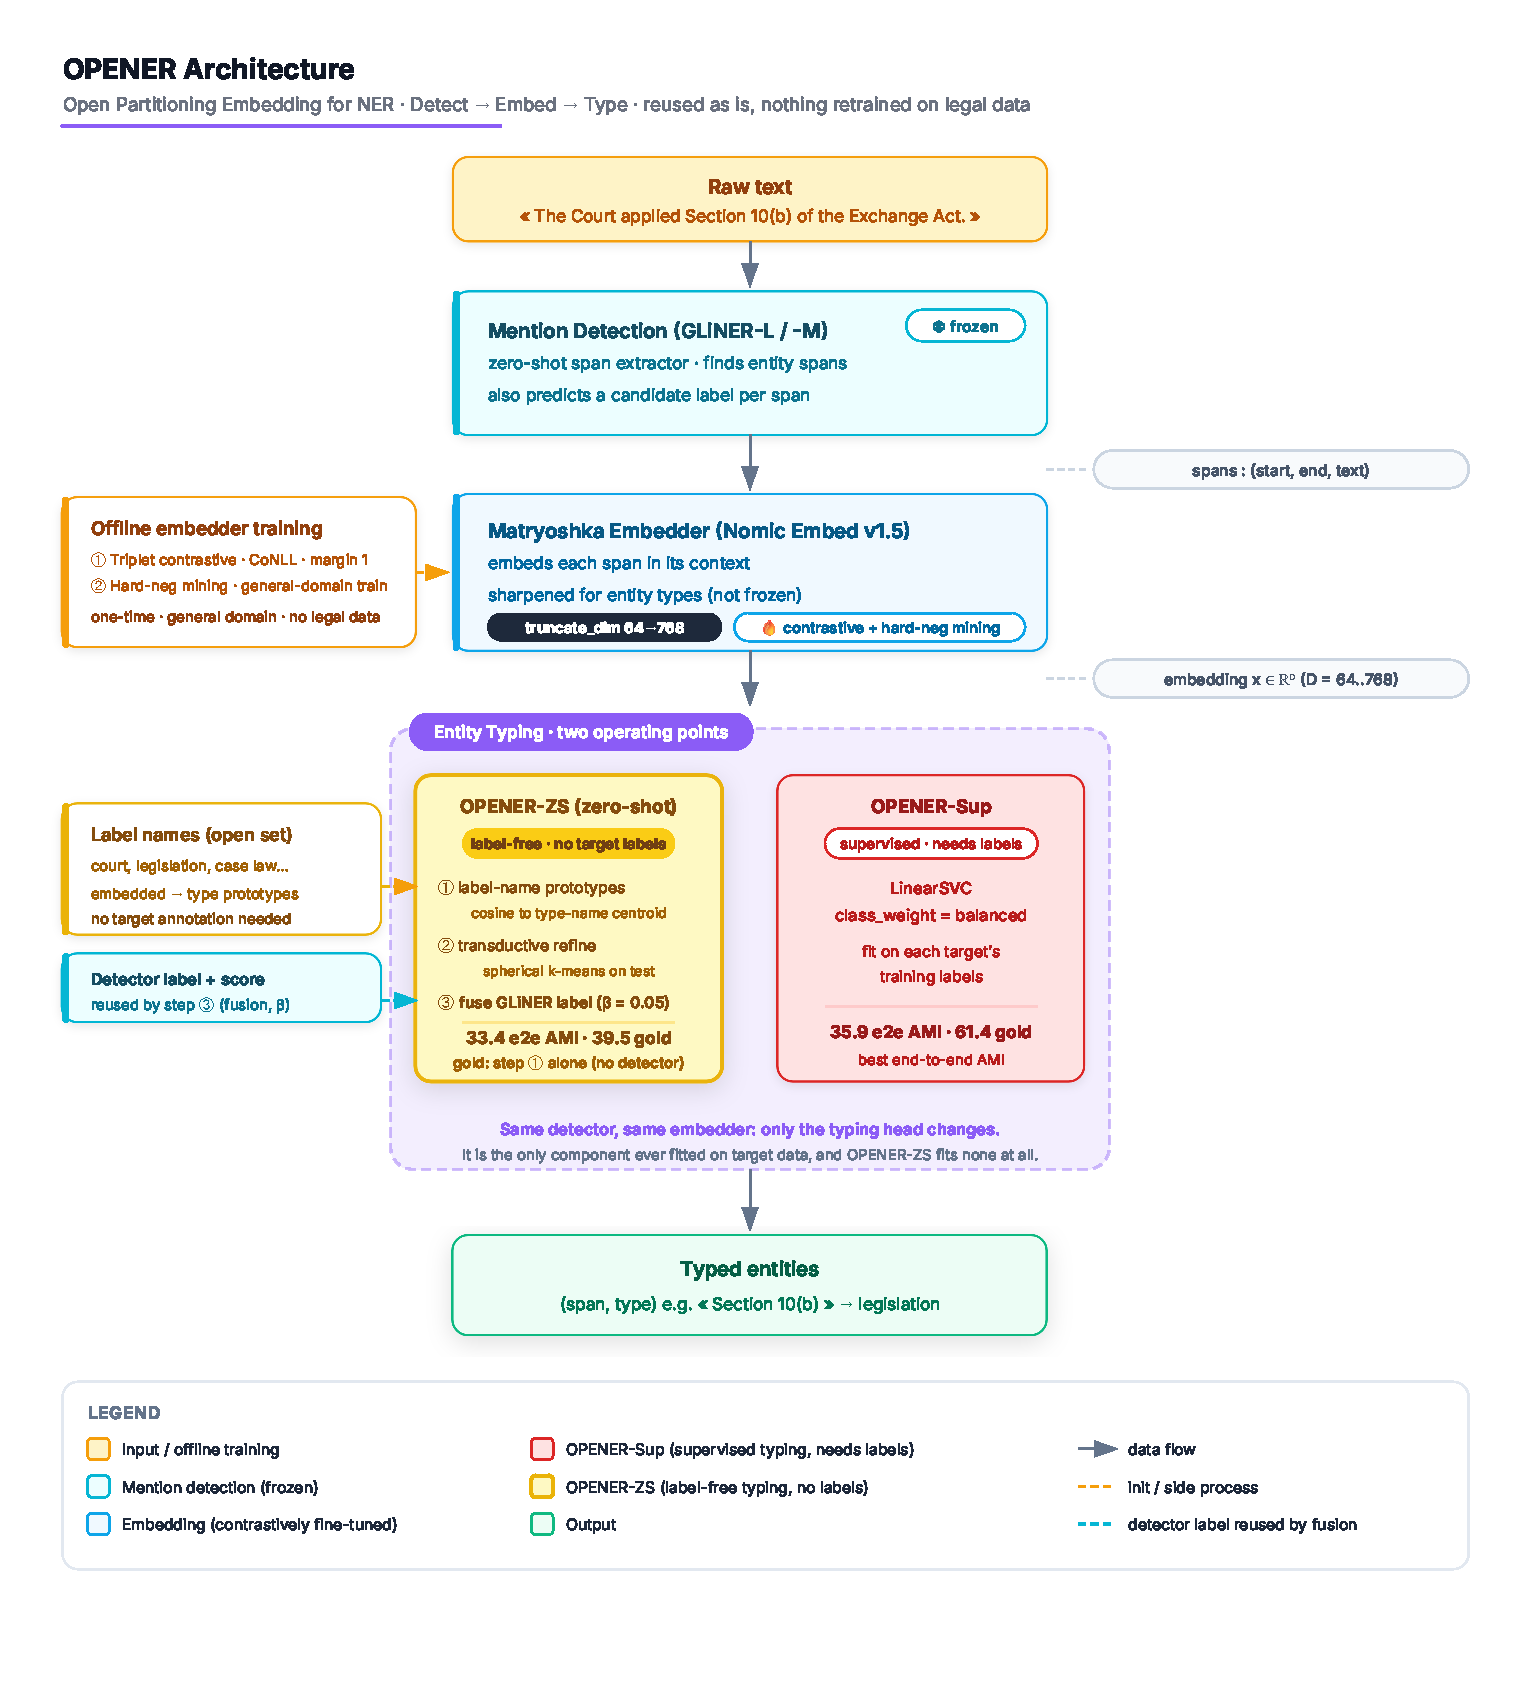
\includegraphics[width=0.52\linewidth]{assets/opener-architecture-v3.pdf}%
}{\IfFileExists{../assets/opener-architecture-v3.pdf}{%
  
\includegraphics[width=0.52\linewidth]{../assets/opener-architecture-v3.pdf}%
}{\fbox{\parbox{0.9\linewidth}{\centering architecture figure (opener-architecture-v3.pdf)}}}}
\caption{The OPENER pipeline (Detect\,$\rightarrow$\,Embed\,$\rightarrow$\,Type), with no component fitted to legal data, with its two typing heads: OPENER-ZS (label-name prototypes, transductive refinement, detector fusion) and OPENER-Sup (supervised linear probe). Nothing is retrained on legal data. The legal AMI figures shown are means over the three embedder-retraining seeds. The end-to-end ones use the full OPENER-ZS head, the typing-on-gold ones its first step alone, since no detector is in the loop (\autoref{sec:exp:setup}).}
\label{fig:pipeline}
\end{figure*}

\subsection{\rev{Overview and notation}}
\label{sec:method:overview}
\rev{The pipeline runs in three stages, and \autoref{fig:pipeline} shows them in order.} The detector maps a sentence $s$ to a set of candidate mentions $\mathcal{M}(s)=\{m_i\}$, each mention is embedded \emph{in context}, and a typing head assigns it a type drawn from the target inventory $\mathcal{T}$,
\begin{equation}
e_i = f_\theta(s, m_i)\in\mathbb{R}^{D},\qquad \hat y_i\in\mathcal{T},
\end{equation}
where $f_\theta$ is the frozen embedder and $e_i$ the $D$-dimensional vector it produces for mention $m_i$, read together with its sentence $s$. We keep the full $D{=}768$. The predicted type $\hat y_i$ is drawn from $\mathcal{T}$, the legal type inventory of the target corpus, which $f_\theta$ never saw during its own training. \rev{Stages one and two are identical at both operating points. Only the typing head of stage three changes, and \autoref{tab:protocols} in \autoref{sec:appendix:protocols} states exactly how.}

\subsection{\rev{Preprocessing}}
\label{sec:method:preprocessing}
\rev{Three preparation steps sit between a raw legal corpus and the pipeline, and each one is a deliberate choice rather than a formatting detail.}

\rev{\paragraph{Corpus normalisation} The four corpora ship in different formats (CoNLL columns, character spans, token-level tags). We convert them all to one representation, a sentence paired with $(\text{start},\text{end},\text{type})$ triples in \emph{character} offsets, so a single evaluation path serves every corpus and no system benefits from a corpus-specific reader. Sentences with no gold entity are dropped, on every system alike, and each test split is capped at its first $1000$ entity-bearing sentences.}

\rev{\paragraph{Span-in-context encoding} The embedder never sees a mention in isolation. A mention spanning characters $[a,b)$ of sentence $s$ is encoded as the whole sentence with the mention delimited in place,}
\rev{\begin{equation*}
\texttt{classification:}\;s_{<a}\;\texttt{[ENT]}\;s_{a:b}\;\texttt{[/ENT]}\;s_{\geq b},
\end{equation*}}
\rev{where \texttt{classification:} is the task prefix Nomic v1.5 expects. Keeping the sentence is what lets the same surface form be typed differently in two contexts, which legal text demands constantly (a party name that is a company in one clause and a litigant in the next). The markers, rather than a cropped span, keep that context while still telling the encoder which tokens to describe.}

\rev{\paragraph{Type anchors} OPENER-ZS needs a vector per type, and a raw schema code such as \texttt{ORGANIZACAO} or \texttt{GS} carries little meaning for an English-trained encoder. Each type therefore receives one to five English anchor words (\texttt{COURT} $\rightarrow$ \emph{court}, \emph{tribunal}, \emph{judiciary}), listed in full in \autoref{sec:appendix:setup} and fixed before any result was seen. End-to-end, every anchor is embedded through the same four templates, \emph{\{a\}}, \emph{a \{a\}}, \emph{the \{a\}} and \emph{an example of \{a\}}, each one passed through the span-in-context format above with the anchor itself marked. The point is distributional: a prototype built this way is produced by the same input format as the mentions it will be compared against, instead of a bare word the encoder would see in a format it never meets at inference.}

\subsection{\rev{Mention detection}}
\label{sec:method:detection}
Spans are proposed by a frozen GLiNER detector \citep{zaratiana2024gliner} \rev{prompted with the target type names at confidence threshold $0.3$, the value released with the model. The two heads run on different sizes, GLiNER-L for OPENER-ZS and GLiNER-M for OPENER-Sup, because the detector is a modular slot rather than a tuned hyperparameter. \autoref{tab:legal-main} reports every GLiNER size on its own, so the effect of that choice stays readable from the baselines rather than hidden inside our pipeline.}

\subsection{\rev{Entity embedding}}
\label{sec:method:embedding}
Mentions are embedded by Nomic v1.5 \citep{nussbaum2024nomic}, a Sentence-BERT-style \citep{reimers2019sbert}, Matryoshka-truncatable embedder \citep{kusupati2022matryoshka} that we sharpen once, with a FaceNet triplet step \citep{schroff2015facenet} on English, general-domain CoNLL-2003 \citep{tjongkimsang2003conll} spans and an error-driven hard-negative mining pass. Training it away from any legal schema is deliberate, and the same single checkpoint then serves all four legal schemas here without re-fitting. Nothing in the pipeline is legal-specific except the type inventory it is asked about, and that is exactly the design this paper puts to the test. \rev{We keep the full $768$ dimensions and use no Matryoshka truncation, since the embedder is not the cost bottleneck of the pipeline (\autoref{tab:legal-main}) and truncating would trade quality for a saving we do not need.}
\rev{Both embedder checkpoints are public.\footnote{\scriptsize\url{https://huggingface.co/Thibault-GAREL/opener-sup} and \url{https://huggingface.co/Thibault-GAREL/opener-zs}.}}

\subsection{Entity typing}
\label{sec:method:typing}
\paragraph{OPENER-ZS} The zero-shot head, the open-world default, uses no target labels. Each legal type $t$ is represented by a prototype $p_t$, the $\ell_2$-normalised centroid of the embeddings of the words forming its name,
\begin{equation}
\begin{split}
\overline{e}_t&=\frac{1}{|\mathrm{name}(t)|}\!\!\sum_{w\,\in\,\mathrm{name}(t)}\!\!f_\theta(w),\\[2pt]
p_t &= \overline{e}_t\,\big/\,\lVert \overline{e}_t\rVert_2,
\end{split}
\end{equation}
where $\mathrm{name}(t)$ is the set of anchor words naming type $t$ (\autoref{sec:method:preprocessing}). Each anchor word $w$ contributes its embedding $f_\theta(w)$, and $\overline{e}_t$ is their average. Dividing that average by its Euclidean norm $\lVert\overline{e}_t\rVert_2$ gives a unit-length prototype. \rev{End-to-end, $f_\theta(w)$ is replaced by the four-template average of \autoref{sec:method:preprocessing}, which changes the vector but not the equation.}

A mention is assigned the nearest prototype by cosine similarity, refined by a \emph{transductive} pass of spherical $k$-means over the unlabelled test mentions, seeded by the prototypes, and \emph{fused} with the detector's own zero-shot label,
\begin{equation}
s_t(i)=\cos(e_i,\tilde{p}_t)+\beta\,g_i\,\indic\!\left[t=\ell_{\text{GLiNER}}(i)\right],
\end{equation}
where $s_t(i)$ is the fused score of assigning type $t$ to mention $m_i$, and $\tilde{p}_t$ the centroid of type $t$ after that refinement, which is $p_t$ itself when the transductive pass is switched off. The detector contributes the type $\ell_{\text{GLiNER}}(i)$ it predicted for that span and its confidence $g_i\in[0,1]$ in it. The indicator $\indic[\cdot]$ is worth $1$ only when $t$ is that predicted type, so the fusion term only ever raises the score of the detector's own choice, and the mention is typed as $\hat y_i=\arg\max_t s_t(i)$. \rev{Two constants govern this head, and both are fixed a priori rather than tuned on a legal set. The refinement runs three iterations, enough for the centroids to settle on corpora of this size and few enough to keep them anchored to the label names that seeded them. The fusion weight $\beta{=}0.05$ is small on purpose, so the detector can only break ties the prototypes leave open instead of overriding them, a bound \autoref{sec:appendix:beta} then sweeps post-hoc.}

\paragraph{OPENER-Sup} A balanced linear classifier (scikit-learn's LinearSVC \citep{pedregosa2011scikit} with \texttt{class\_weight=balanced}, built on LIBLINEAR \citep{fan2008liblinear}) is fit one-vs-rest on the legal target's training labels. For each type $c$, it minimises a squared-hinge objective with balanced class weights,
\begin{equation}
\begin{split}
\min_{w_c,b_c}\;&\tfrac12\lVert w_c\rVert_2^2\\
&+\,C\sum_i \omega_{y_i}\,\max\!\big(0,\,1-z_{ic}\,h_c(e_i)\big)^2,
\end{split}
\end{equation}
with $h_c(e_i)=w_c^{\top} e_i+b_c$ the one-vs-rest hyperplane of type $c$, $e_i$ the frozen embedding of training mention $i$, $y_i$ its gold legal type, $z_{ic}={+}1$ if $y_i{=}c$ and ${-}1$ otherwise, and $C$ the regularisation strength. The balancing weight $\omega_c=n/(|\mathcal{T}|\,n_c)$ up-weights rare types, with $n$ the total number of training mentions and $n_c$ the count of type $c$. This matters on legal schemas, where a single type can hold well under $1\%$ of the mentions (Court in E-NER, \autoref{tab:legal-datasets}). A mention is typed as $\hat y_i=\arg\max_c h_c(e_i)$. Rather than a single label-name match, this carves the embedding space into one region per type, separating types whose vectors sit close together as long as their regions do not overlap. This is the supervised upper bound, and it needs target labels. \rev{End-to-end the probe is fit on the detector's own training spans rather than on gold ones, so that it learns to type the noisy boundaries it will actually be handed at inference.}

\subsection{\rev{Evaluation protocol}}
\label{sec:method:evaluation}
We report both \emph{typing-on-gold} (perfect detection) and \emph{end-to-end} protocols. Predicted and gold mentions are aligned by exact character offsets, and detection errors stay in the evaluation through sentinel labels, one for a gold mention no system predicted and one for a predicted span with no gold counterpart, following the alignment protocol of \citet{genest2025owner}. Sentences carrying no gold entity are not evaluated, on any system.

\paragraph{\rev{Quality}} Quality is the Adjusted Mutual Information (AMI) \citep{vinh2010ami} between the gold type partition $U$ and the predicted partition $V$ over the aligned mentions,
\begin{equation}
\mathrm{AMI}=\frac{\mathrm{MI}-\mathbb{E}\!\left[\mathrm{MI}\right]}{\tfrac12\!\left[H(U)+H(V)\right]-\mathbb{E}\!\left[\mathrm{MI}\right]},
\end{equation}
where $\mathrm{MI}=\mathrm{MI}(U,V)$ is the mutual information between the two partitions, which measures how much a mention's predicted type reduces the uncertainty about its gold type, and $H$ the entropy. Subtracting the chance agreement $\mathbb{E}[\mathrm{MI}]$ makes a random typing score near $0$ whatever the number of types, a perfect one $1$. The denominator uses the arithmetic-mean normalisation (the scikit-learn default). \rev{We report it as AMI\,$\times100$, so the scale runs from ${\approx}0$ for chance to $100$ for a partition identical to the gold one. The value $100$ is reachable in the typing-on-gold protocol, where both partitions cover the same mentions, but end-to-end it is not: a missed or spurious span puts a sentinel on one side and a real type on the other, so any detection error caps the score below $100$ whatever the typing head does. \autoref{sec:exp:results} quantifies that cap directly.}

\rev{\paragraph{Why AMI, and what we report beside it} AMI is invariant to a relabelling of the predicted types: a system that consistently called \emph{judges} what the gold calls \emph{lawyers}, and conversely, would score $100$ AMI and $0$ F1. That invariance is the point here, since OWNER names its clusters dynamically and the generative baselines paraphrase type strings, so a metric requiring predicted and gold names to coincide cannot score them at all. AMI is also corrected for chance, which matters across schemas of $6$ to $19$ unequally frequent types. The argument binds only for systems answering outside the target inventory, though. OPENER's heads, the GLiNER family, GNER and the LLM baseline all answer inside it, so for these an F1 is well defined and we report it: macro-F1 on gold mentions (\autoref{tab:legal-gold}) and micro entity-level precision, recall and F1 end-to-end (\autoref{tab:legal-decomp}), a span counting as correct only when offsets and type both match, the convention of the four dataset papers. OWNER alone has none.}

\paragraph{\rev{Cost}} We also report per-sentence latency (p50) and energy (Wh per $1000$ sentences, measured with CodeCarbon \citep{codecarbon2024}).

\section{Experiments}
\label{sec:experiments}

\subsection{Datasets}
\label{sec:exp:datasets}
We evaluate on four legal-specific NER sets across three languages that, together, separate two kinds of distribution shift. \emph{Two are in English}, isolating a \emph{pure domain shift} from the general-domain spans the embedder was fine-tuned on: E-NER \citep{au2022ener} (U.S.\ SEC/EDGAR filings, $7$ types) and Indian-Legal \citep{kalamkar2022indianlegal} (Indian court judgements, $14$ fine-grained legal types). LeNER-Br \citep{luzdearaujo2018lenerbr} (Brazilian court decisions) and German-LER \citep{leitner2020germanler} (German federal court decisions) add a \emph{cross-lingual} shift. All four annotate \emph{legal-specific} types (courts, statutes, legislation, case law, provisions) rather than the generic person/organisation/date schema of general NER. \rev{\autoref{tab:legal-datasets} in \autoref{sec:appendix:datasets} gives their sizes, along with the supervised topline published with each one, from $91.1$ to $96.1$ entity-level F1. Those figures set the scale our end-to-end numbers should be read against.}


\subsection{Setup}
\label{sec:exp:setup}
Embedder, detector and heads are exactly those of \autoref{sec:method}, and nothing is retrained on legal data. The baselines are GLiNER-S/M/L, GNER-T5-base, OWNER and \rev{an instruction-tuned LLM baseline, Qwen2.5-1.5B-Instruct in $4$-bit}, all prompted zero-shot with the target type names. Test splits are capped at the first $1000$ entity-bearing sentences, with Qwen on a $200$-sentence subsample. \rev{That model is the largest our $6$\,GB GPU runs, and a hosted frontier model would have made the latency and energy axes unmeasurable, a constraint we spell out in the Limitations.}

\autoref{tab:legal-setup} in \autoref{sec:appendix:setup} gives the complete configuration. Every typing hyperparameter of \autoref{sec:method} is fixed a priori and never tuned on a legal set, $C{=}1$ for the balanced probe included. \rev{Evaluation code, anchor dictionaries, dataset loaders and per-run logs are public.\footnote{\scriptsize\url{https://github.com/Thibault-GAREL/LyRIDS_Law-OPENER}}}
% Les URLs sont desormais dans le texte ci-dessus (footnote). Datasets publics,
% charges par src/data/legal_datasets.py.

The two protocols do not exercise the same zero-shot head (\autoref{tab:protocols}): \autoref{tab:legal-gold} measures the label-name geometry on its own, \autoref{tab:legal-main} the operating point one would deploy.

We report two orthogonal sources of uncertainty. The embedder's \emph{training} is stochastic, so the study is repeated under three retraining seeds, every OPENER cell giving mean\,$\pm$\,std, the baselines being frozen checkpoints run once. Inference being deterministic, the remaining uncertainty is the finite test set, quantified with a paired bootstrap in \autoref{sec:exp:results}. Efficiency is deliberately \emph{not} seed-averaged, since a seed changes the embedder's weights and not its per-sentence FLOPs.

\subsection{Results}
\label{sec:exp:results}
Keeping the two protocols apart, \autoref{tab:legal-gold} reports typing-on-gold quality and \autoref{tab:legal-main} the end-to-end comparison. OWNER appears in both, as the one baseline that types mentions it is given rather than detecting and typing jointly. Three findings stand out.

\textbf{Label-free typing is strong in English but degrades cross-lingually.} OPENER-ZS is usable on the two English sets ($47.7$ on E-NER and $49.1$ on Indian, from English label-name prototypes alone), but it drops to $37.4$ (pt) and $23.8$ (de). Its English prototypes align well with English legal mentions, far less with other-language ones (\autoref{tab:legal-gold}). It also trails OWNER's own label-free typing on all four sets ($44.7$ mean against $39.5$). OWNER trains an entity encoder rather than reusing one, so the label-free operating point is where reuse costs the most. It is also the \emph{seed-sensitive} head. Its gold scores vary by ${\pm}3$--$6$ AMI across the three embedder retrainings, and the released one is in fact a low draw on the English sets, whereas the supervised probe varies by at most ${\pm}1.4$. Label-name prototypes depend on the fine geometry of the embedding space, which shifts from one contrastive retraining to the next, while a fitted probe absorbs those shifts.

\textbf{Supervised typing transfers well, including across languages, because the separation it learns is geometric, not just statistical.} Fitting a balanced linear probe on the same frozen, general-domain embedder reaches $61.4$ mean typing-on-gold AMI over the four sets. That is $70.9$ and $60.8$ on the two English corpora, and still $53.7$ and $60.3$ on Portuguese LeNER-Br and German-LER, with a spread of at most ${\pm}1.4$ AMI across seeds. It leads OWNER on every set, by $16$ AMI on E-NER and by $35$ on German. It also scores $62.3$ in a preliminary general-domain check (ongoing work), so keeping the space unspecialised costs under a point of AMI here. A balanced probe fits hyperplanes precise enough to pull apart legal types whose vectors sit \emph{close together}, a lawyer from a judge, or a statute from a case citation. A single label-name match cannot draw that boundary without supervision. \rev{Macro-F1 over the same gold predictions tells the same story ($89.1$ on E-NER, $74.6$ on average, against $46.1$ for the label-free head), so no conclusion here hinges on the choice of metric. Those figures type mentions that are given, whereas the published toplines of \autoref{sec:exp:datasets} include detection, so the two are not two sides of one comparison. What the pair does show is that typing is not where a frozen, general-domain space falls short.}

\textbf{End-to-end, detection sets the ceiling, and the label-free head cannot pull ahead of the detector it fuses with.} On these legal-specific schemas, every system clusters in a narrow $\approx 33$--$36$ AMI band (\autoref{tab:legal-main}), because the English detectors recover only a fraction of gold mentions (GLiNER-L offset recall $18.7$--$57.4\%$, GLiNER-M $10.2$--$61.1\%$). With so few mentions detected, no typing head can pull far ahead. Per-dataset winners are specific, OWNER \citep{genest2025owner} on E-NER and GNER-T5 on German, though OWNER degrades most across languages at several times the cost of either OPENER head. Qwen trails throughout, while being the most energy-hungry per sentence. \emph{Averaged over the four sets, OPENER-Sup posts the best end-to-end AMI ($35.9$)}, narrowly ahead of GLiNER-L ($35.0$) and GLiNER-M ($34.9$), for every retraining seed. OPENER-ZS ($33.4$) sits just below OWNER ($33.7$). The margins are small, as expected when detection is the ceiling. A \emph{paired} bootstrap on the released model ($K{=}1000$) nonetheless makes OPENER-Sup's lead \textbf{statistically significant}, at $+1.0$ AMI over both GLiNER-M and GLiNER-L ($95\%$ CI $[+0.4,+1.7]$ and $[+0.1,+1.9]$). OPENER-ZS's fusion sits significantly \emph{below} GLiNER-L ($-1.3$, $[-1.8,-0.8]$), largely deferring to the detector's labels.

\begin{table}[tbp]
\centering
\caption{Typing-on-gold quality (${\times}100$, $\uparrow$)\rev{, in AMI and macro-F1}.}
\label{tab:legal-gold}
\scriptsize
\setlength{\tabcolsep}{1.5pt}
\begin{threeparttable}
\begin{tabular}{@{}l@{\hskip 7pt}ccccc@{}}
\toprule
System & E-NER & Indian & LeNER-Br & German & Mean \\
       & (en)  & (en)   & (pt)     & (de)   &      \\
\midrule
\multicolumn{6}{l}{\emph{AMI}} \\
OWNER$^\S$ & $54.5$ & $59.0$ & $39.7$ & $25.7$ & $44.7$ \\
\rowcolor{hlyellow} OPENER-ZS & $47.7_{\pm3.5}$ & $49.1_{\pm3.0}$ & $37.4_{\pm6.0}$ & $23.8_{\pm4.3}$ & $39.5_{\pm3.0}$ \\
\rowcolor{hlred} OPENER-Sup$^\ast$   & $\mathbf{70.9}_{\pm1.2}$ & $\mathbf{60.8}_{\pm1.4}$ & $\mathbf{53.7}_{\pm1.2}$ & $\mathbf{60.3}_{\pm1.0}$ & $\mathbf{61.4}_{\pm0.4}$ \\
\addlinespace
\multicolumn{6}{l}{\rev{\emph{Macro-F1} (OWNER: n/a$^\dagger$)}} \\
\rowcolor{hlyellow} \rev{OPENER-ZS} & \rev{$59.2_{\pm7.0}$} & \rev{$37.6_{\pm5.3}$} & \rev{$57.7_{\pm6.0}$} & \rev{$29.7_{\pm5.4}$} & \rev{$46.1_{\pm5.3}$} \\
\rowcolor{hlred} \rev{OPENER-Sup$^\ast$} & \rev{$\mathbf{89.1}_{\pm0.2}$} & \rev{$\mathbf{58.3}_{\pm2.5}$} & \rev{$\mathbf{74.7}_{\pm1.5}$} & \rev{$\mathbf{76.3}_{\pm1.3}$} & \rev{$\mathbf{74.6}_{\pm0.3}$} \\
\bottomrule
\end{tabular}
\begin{tablenotes}[flushleft]
\scriptsize
\item Typing on gold mentions, detection bypassed. OPENER cells: mean\,$\pm$\,std over three embedder-retraining seeds (\autoref{sec:exp:setup}), test-set bootstrap std ${\pm}0.8$--$1.7$ AMI. Best per column in bold, within each block.
\item[$\ast$] Only OPENER-Sup uses target labels. $^\S$\,OWNER typing its own clusters, single deterministic run of the released checkpoint, zero-shot transfer as in \autoref{tab:legal-main}.
\item[$\dagger$] \rev{OWNER names its clusters dynamically, so its predictions carry no label from the target inventory and no F1 can be computed against it. This is the one case the argument of \autoref{sec:method:evaluation} actually binds, and the reason AMI is our primary axis.}
\end{tablenotes}
\end{threeparttable}
\end{table}

\begin{table}[tbp]
\centering
\caption{Open-world legal NER, end-to-end\rev{: quality on each corpus}.}
\label{tab:legal-main}
\scriptsize
\setlength{\tabcolsep}{1.5pt}
\begin{threeparttable}
\begin{tabular}{@{}l@{\hskip 7pt}ccccc@{}}
\toprule
Model & E-NER & Indian & LeNER-Br & German & Avg \\
      & (en)  & (en)   & (pt)     & (de)   &     \\
\midrule
\multicolumn{6}{l}{\emph{AMI} ($\times100$, $\uparrow$), zero-shot} \\
GLiNER-S & $33.4$ & $33.9$ & $33.7$ & $31.1$ & $33.0$ \\
GLiNER-M & $33.9$ & $34.8$ & $34.8$ & $36.1$ & $34.9$ \\
GLiNER-L & $34.7$ & $\mathbf{35.2}$ & $\mathbf{36.3}$ & $34.0$ & $\mathbf{35.0}$ \\
GNER-T5  & $28.7$ & $28.6$ & $33.2$ & $\mathbf{39.2}$ & $32.4$ \\
Qwen-1.5B$^\ddagger$ & $24.9$ & $28.1$ & $24.9$ & $14.5$ & $23.1$ \\
OWNER$^\S$ & $\mathbf{38.4}$ & $33.3$ & $34.8$ & $28.4$ & $33.7$ \\
\rowcolor{hlyellow} OPENER-ZS & $33.4_{\pm0.2}$ & $33.8_{\pm0.5}$ & $33.5_{\pm1.2}$ & $32.8_{\pm0.4}$ & $33.4_{\pm0.4}$ \\
\addlinespace[1pt]
\multicolumn{6}{l}{\emph{AMI}, with target labels} \\
\rowcolor{hlred} OPENER-Sup$^\ast$ & $35.7_{\pm0.3}$ & $35.2_{\pm0.3}$ & $34.1_{\pm0.7}$ & $38.5_{\pm0.3}$ & $\mathbf{35.9}_{\pm0.4}$ \\
\bottomrule
\end{tabular}
\begin{tablenotes}[flushleft]
\scriptsize
\item Detector mentions, offset/sentinel alignment (\autoref{sec:exp:setup}). Best per column in bold, within each block, ties included, the two AMI sub-blocks bolded apart since OPENER-Sup is the only row that consumes target labels. OPENER rows are mean\,$\pm$\,std over three retraining seeds, baselines are frozen checkpoints with a single deterministic run. \rev{Model size and cost in \autoref{tab:legal-efficiency}, per-corpus cost in \autoref{tab:legal-cost-detail}.}
\item[$\ast$] Only OPENER-Sup uses target labels, every other row is zero-shot. $^\ddagger$\,Qwen AMI on a $200$-sentence subsample. $^\S$\,OWNER typing its own dynamically named clusters.
\end{tablenotes}
\end{threeparttable}
\end{table}

\subsection{Analysis}
\label{sec:exp:analysis}
Two distribution shifts act together here, and the results separate them. Under a pure \emph{domain} shift (E-NER), the unspecialised embedder already places legal types far enough apart for a label-name prototype to separate them ($47.7$ gold AMI, with no target label at all). A cross-lingual shift widens the gap, the label-free head dropping to $24$--$37$ while the probe stays high ($53.7$/$60.3$).

A stress test on German-LER's fine $19$-type schema isolates fineness of separation from language. OPENER-ZS falls to $22.7_{\pm2.1}$ gold AMI there, as fine German type codes rarely have a faithful English prototype. OPENER-Sup still reaches $61.5_{\pm0.7}$, \emph{on a par with its coarse score} ($60.3$) despite nearly three times as many classes. The zero-shot weakness is therefore not the embedding geometry, but the missing supervised signal.

Language alone does not explain the collapse of detection on German. GLiNER-L recovers $43.9\%$ of the Portuguese mentions, on a par with the $44.5\%$ it reaches on English Indian judgements, and only German collapses. Its schema is as singular as its language, since legal-norm and case-law citations make up $62\%$ of its mentions, and both are long multi-token strings. Either way, an in-language \emph{detector} would lift the ceiling far more than a better typing head. Within our frugal, retraining-free budget, OPENER-Sup is therefore the practical default wherever even a modest labelled sample exists.

\rev{\textbf{Where end-to-end quality is actually lost.} \autoref{tab:legal-decomp} splits each end-to-end score into its two stages, the rows of a pair differing \emph{only} in the typing head. The supervised head is then worth more than its $+1.0$ AMI suggests. On correctly detected mentions, it types $78.7\%$ right, against the detector's own $64.6\%$. That $14$-point gain is hidden by the average, because it applies only to the $35.7\%$ of mentions that survive detection. The zero-shot head moves the other way, $64.5\%$ against $70.1\%$, which is why its fusion sits below the detector it fuses with. Typing those same spans \emph{perfectly} reaches only ${\approx}70$ AMI, so a third of the scale is out of reach before typing even begins. That bound is itself generous, since it credits the oracle with telling a spurious span from a real one, which is detection work.}

\begin{table}[tbp]
\centering
\caption{\rev{End-to-end quality split into its two stages, four-set means (${\times}100$). An arrow marks a head running \emph{on} the detector above it, so the two rows share their detected spans and differ only in the typing head.}}
\label{tab:legal-decomp}
\scriptsize
\setlength{\tabcolsep}{2pt}
\begin{threeparttable}
\begin{tabular}{@{}l@{\hskip 7pt}cccccc@{}}
\toprule
System & \multicolumn{2}{c}{Detection} & Typing & \multicolumn{3}{c}{End-to-end} \\
\cmidrule(lr){2-3}\cmidrule(lr){4-4}\cmidrule(lr){5-7}
 & exact & touched & acc. & F1 & AMI & oracle \\
\midrule
GLiNER-S & $34.4$ & $55.1$ & $62.2$ & $22.2$ & $33.0$ & $65.9$ \\
GNER-T5 & $39.8$ & $77.2$ & $56.5$ & $18.4$ & $32.4$ & $74.2$ \\
Qwen-1.5B$^\ddagger$ & $14.2$ & $20.5$ & $68.2$ & $10.4$ & $23.1$ & $42.2$ \\
OWNER$^\S$ & n/a & n/a & n/a & n/a & $33.7$ & n/a \\
\addlinespace[2pt]
\multicolumn{7}{l}{\emph{Same detector, different typing head}} \\
GLiNER-L & $41.1$ & $68.6$ & $70.1$ & $25.0$ & $35.0$ & $72.0$ \\
\rowcolor{hlyellow} \hspace{4pt}$\hookrightarrow$ OPENER-ZS & $41.1$ & $68.6$ & $64.5$ & $23.1$ & $33.7$ & $72.0$ \\
\addlinespace[1pt]
GLiNER-M & $35.7$ & $63.4$ & $64.6$ & $22.8$ & $34.9$ & $69.8$ \\
\rowcolor{hlred} \hspace{4pt}$\hookrightarrow$ OPENER-Sup$^\ast$ & $35.7$ & $63.4$ & $\mathbf{78.7}$ & $\mathbf{25.3}$ & $\mathbf{35.9}$ & $69.8$ \\
\bottomrule
\end{tabular}
\begin{tablenotes}[flushleft]
\scriptsize
\item \rev{\emph{exact}: gold mentions recovered on both offsets (the recall of \autoref{sec:exp:results}). \emph{touched}: also counting mentions a prediction overlaps without matching their boundaries. \emph{acc.}: share of exactly detected mentions given the right type, which isolates the typing head. \emph{F1}: micro entity-level, offsets and type both correct. \emph{oracle}: the ceiling these detected spans allow, each correctly detected span taking its gold type and every spurious span a single shared label. It is a function of the detector alone, hence identical within a pair, and it is a \emph{loose} upper bound, since recognising a span as spurious is detection rather than typing. Every figure here is the released seed alone, so the AMI column can differ slightly from the three-seed means of \autoref{tab:legal-main} ($33.7$ against $33.4$ for OPENER-ZS, for instance).}
\item[$\ast$] \rev{Only OPENER-Sup uses target labels.} $^\ddagger$\,\rev{Qwen on a $200$-sentence subsample per corpus.} $^\S$\,\rev{OWNER cannot be decomposed here for two independent reasons: it names its clusters dynamically, so neither typing accuracy nor F1 is defined against the target inventory, and it aligns mentions by word index rather than by character offset, so its detection columns would not be commensurable with the rest of the table. Its AMI is repeated from \autoref{tab:legal-main} for reference.}
\end{tablenotes}
\end{threeparttable}
\end{table}

\rev{\textbf{Most detection failures are boundaries, not blindness.} Counting a mention as \emph{touched} when a prediction overlaps it without matching both offsets, GLiNER-L touches $68.6\%$ of gold mentions but aligns only $41.1\%$ exactly, and the generative baseline is the extreme case at $77.2\%$ against $39.8\%$ (\autoref{tab:legal-decomp}). German is the one corpus this does not rescue, GLiNER-L reaching $38.4\%$ there even relaxed. Cross-lingual transfer and long-span detection were confounded in that corpus, and this separates them. German fails as a language, not only as a schema of long spans.}

\rev{\textbf{What the two heads confuse.} The confusions are exactly the ones the design predicts (\autoref{sec:appendix:errors}). On German-LER, OPENER-ZS maps \textsc{norm} onto \textsc{regulation} $213$ times, its dominant error by far, where the probe makes that same confusion $3$ times, the two anchor names being near-synonyms in English while the corpus separates the types sharply. On Indian-Legal it collapses \textsc{other-person} into procedural roles $123$ times, which no label-name prototype can avoid, since those types all name people. Supervision, not a better embedder, is what the label-free head lacks.}

\rev{\textbf{Quality against cost.}} \autoref{tab:legal-efficiency} closes the picture, with every axis on one row per system. Both heads match the frugal GLiNER family in cost, one to two orders of magnitude below the generative baselines and several times below OWNER. OPENER-Sup does so while leading on \rev{both quality measures}, at $337$M parameters against OWNER's $294$M and Qwen's $1.5$B. Quality and cost are not traded off against each other here.

\begin{table}[tbp]
\centering
\caption{\rev{Quality against cost}, four-set means of \autoref{tab:legal-main} \rev{and \autoref{tab:legal-decomp}}.}
\label{tab:legal-efficiency}
\scriptsize
\setlength{\tabcolsep}{3pt}
\begin{threeparttable}
\begin{tabular}{@{}l@{\hskip 5pt}rrrrr@{}}
\toprule
Model & Params & AMI\,$\uparrow$ & \rev{F1\,$\uparrow$} & p50 (ms)\,$\downarrow$ & Energy (Wh)\,$\downarrow$ \\
\midrule
\multicolumn{6}{l}{\emph{Zero-shot (no target labels)}} \\
GLiNER-S & $50$M & $33.0$ & \rev{$22.2$} & $\mathbf{22}$ & $\mathbf{0.5}$ \\
GLiNER-M & $200$M & $34.9$ & \rev{$22.8$} & $37$ & $0.7$ \\
GLiNER-L & $330$M & $\mathbf{35.0}$ & \rev{$\mathbf{25.0}$} & $81$ & $1.6$ \\
GNER-T5 & $220$M & $32.4$ & \rev{$18.4$} & $8289$ & $96.0$ \\
Qwen-1.5B$^\ddagger$ & $1.5$B & $23.1$ & \rev{$10.4$} & $5426$ & $100.5$ \\
OWNER$^\S$ & ${\approx}294$M & $33.7$ & \rev{n/a$^\dagger$} & $475$ & $14.6$ \\
\rowcolor{hlyellow} OPENER-ZS & $467$M & $33.4_{\pm0.4}$ & \rev{$23.1$} & $133$ & $2.7$ \\
\addlinespace[1pt]
\multicolumn{6}{l}{\emph{With target labels}} \\
\rowcolor{hlred} OPENER-Sup$^\ast$ & $337$M & $\mathbf{35.9}_{\pm0.4}$ & \rev{$\mathbf{25.3}$} & $84$ & $1.7$ \\
\bottomrule
\end{tabular}
\begin{tablenotes}[flushleft]
\scriptsize
\item End-to-end, energy per $1000$ evaluated sentences (multiply by $0.056$ for gCO\textsubscript{2}), measured on the released seed-$42$ run. Best per column in bold, within each sub-block. Params count the whole pipeline, detector plus the $137$M embedder, so OPENER-Sup is lighter than OPENER-ZS only because it runs on GLiNER-M rather than GLiNER-L. \rev{F1 is the micro entity-level score of \autoref{tab:legal-decomp}.}
\item[$\ast$] Only OPENER-Sup uses target labels. $^\ddagger$\,Qwen AMI on a $200$-sentence subsample, its energy over three sets (\autoref{tab:legal-cost-detail}). $^\S$\,OWNER cost is amortised wall-clock. $^\dagger$\,\rev{OWNER names its clusters dynamically, so no F1 is defined against the target inventory (\autoref{tab:legal-decomp}).}
\end{tablenotes}
\end{threeparttable}
\end{table}

\textbf{Fusion weight $\beta$.} \rev{Sweeping $\beta$ post-hoc (\autoref{sec:appendix:beta}) confirms the reading above. The label-free head interpolates from the refined prototypes alone ($32.4$ average AMI at $\beta{=}0$) up to the GLiNER-L labels ($35.0$), reaching a plateau by $\beta{\approx}0.2$. It can therefore do no better end-to-end than the detector it fuses with. The sweep also shows the transductive pass failing to survive the transfer, which makes the label-free components the ones to re-examine first under a domain and language shift.}

\section{Conclusion}
\label{sec:conclusion}

We built OPENER for legal NER, a frugal open-world pipeline assembled from ready-to-use pretrained parts and deliberately kept free of any legal-specific training, and evaluated both of its typing heads on four legal corpora in three languages against the standard open-world baselines.

The two heads diverge sharply on legal text. OPENER-ZS remains a usable label-free option on English legal text, but it does not lead the zero-shot field: here it trails GLiNER-M/L and OWNER on average, on gold mentions as well as end-to-end, and its gold AMI collapses cross-lingually as its English-centric prototypes stop matching target-language mentions. OPENER-Sup is almost unaffected, holding up even on German-LER's fine $19$-type schema, and it posts the best end-to-end AMI on average, a statistically significant lead. The reason is geometric: a balanced probe fits hyperplanes precise enough to pull apart legal types whose vectors sit close together, which a single label-name match cannot do without supervision. \rev{The confusion counts make this concrete: the label-free head maps German \textsc{norm} onto \textsc{regulation} $213$ times, the probe $3$ times.} The supervised head is therefore the safer operating point wherever labels exist, and OPENER-ZS is best reserved for languages close to the embedder's own.

End-to-end quality remains bounded first by mention \emph{detection}, whichever typing head runs behind it. \rev{A typing oracle over the detected spans stops at ${\approx}42$ AMI, and most of what detection misses are boundary disagreements rather than mentions it never sees.} Adapting the detector in-language, rather than the embedder, is the natural next step and preserves the frugal decoupled design. Nothing else in the design is tied to legal text beyond the type names it is asked about: legal NER was the demanding case we built it for, and it holds.

\section*{Limitations}
\rev{\paragraph{Scale of the LLM comparison} Our LLM baseline is a $4$-bit Qwen2.5-1.5B, and it is the largest instruction-tuned model our hardware runs: every system in this paper is measured on one consumer GPU with $6$\,GB of VRAM, which a $7$B model saturates in $4$-bit and a larger one does not fit at all. Frontier models are reachable only through paid APIs, and this study has no funding line for inference credits. That constraint is not only budgetary. A hosted model would break the very comparison this paper is built on, since two of our three axes cannot be measured through an API: latency would fold in network round-trips, provider-side batching and queueing, none of which is a property of the model, and energy could not be measured at all, the serving hardware being neither known nor instrumentable by CodeCarbon. Reporting an API model beside locally measured systems would therefore mean either dropping the cost axes or filling them with numbers that are not comparable. We take the honest consequence: we do not know how close a frontier LLM would come to the topline on these corpora, and the oracle-typing ceiling of \autoref{sec:exp:results} is our model-independent answer to how much room is left above the systems we could measure.}

Test splits are capped at their first $1000$ entity-bearing sentences, which affects German-LER only, and sentences carrying no gold entity are excluded, so precision on entity-free text is never measured. OPENER scores are means over three embedder-retraining seeds: the supervised and end-to-end scores are stable (std ${\leq}1.4$ AMI), but the label-free prototypes vary by up to ${\pm}6$ AMI across retrainings, so single-seed zero-shot numbers should be read with care. Inference is deterministic for a fixed embedder, and test-set bootstraps on the released model confirm both the typing-on-gold scores (std ${\pm}0.8$--$1.7$ AMI) and the significance of OPENER-Sup's end-to-end lead, stable across resampling seeds $42/7/123$. More fundamentally, both the embedder and the detector are English-centric and used without any legal- or language-domain adaptation, which is the design under test here and also its main exposure. The detectors' low cross-lingual recall (on German, $18.7\%$ for GLiNER-L and $10.2\%$ for GLiNER-M) caps end-to-end quality and is the first thing a follow-up should address.

\section*{Ethics Statement}
This work runs and evaluates entity recognition on four publicly released legal NER benchmarks (E-NER over SEC/EDGAR filings, an Indian court-judgement set, LeNER-Br, and German-LER), used only for evaluation and under their original licenses. Legal documents contain personal data such as the names of parties, judges and counsel. We introduce no new annotations and release no data, we only run inference over the existing public test splits, and we report no individual-level content, so the study adds no privacy exposure and makes no attempt at re-identification.

Open-world NER is error-prone, and our own results show recall dropping sharply outside English (as low as $10.2\%$ on German). The pipeline is therefore meant as an assistive tool that surfaces candidate entities for human review, not as a component of automated legal decision-making, where a missed or mistyped entity can carry material consequences. A missed entity is silent, so a human in the loop remains necessary, especially cross-lingually. Finally, a central motivation of this study is energy frugality. We report per-sentence latency and energy alongside accuracy precisely to make the environmental cost of deployment explicit, and to argue for models that are cheap enough to run on modest hardware.

The authors used Claude Code (Anthropic) to scaffold and debug the evaluation scripts and to draft and copy-edit this manuscript. The research question, the experimental design, the choice of baselines and datasets, the execution of all experiments and the interpretation of the results are the authors' own. The authors reviewed and edited all content and take full responsibility for it.


% NB: acl.sty already sets \bibliographystyle{acl_natbib} and \cite -> \citep.
\bibliography{references}

\appendix
\section{\rev{Entity-type distributions}}
\label{sec:appendix:datasets}

\rev{Share (\%) of test mentions per entity type, for the splits evaluated in \autoref{tab:legal-datasets}.}

\begin{table}[H]
\centering
\caption{\rev{Entity types and their share of test mentions.}}
\label{tab:legal-distributions}
\scriptsize
\setlength{\tabcolsep}{3pt}
\begin{threeparttable}
\rev{\begin{tabular}{@{}p{0.20\linewidth}p{0.72\linewidth}@{}}
\toprule
Dataset & Entity types (share \% of test mentions) \\
\midrule
E-NER (en) & Business 41.8, Misc 18.3, Legislation/Act 13.5, Location 11.3, Person 7.6, Government 7.1, Court 0.3 \\
\addlinespace[2pt]
Indian-Legal (en) & Lawyer 16.7, Court 9.3, Respondent 8.8, Other-person 8.7, Provision 8.5, Statute 7.3, Date 7.1, Petitioner 6.0, then GPE, Precedent, Org, Judge, Case-number and Witness, from 5.9 down to 1.9 \\
\addlinespace[2pt]
LeNER-Br (pt) & Organiza\c{c}\~{a}o 32.6, Legisla\c{c}\~{a}o 24.6, Pessoa 15.2, Tempo 12.5, Jurisprud\^{e}ncia 12.0, Local 3.1 \\
\addlinespace[2pt]
German-LER (de) & Legal-norm 38.3, Case-law 23.4, Organization 15.0, Regulation 6.7, Person 6.1, Legal-literature 5.9, Location 4.7 \\
\bottomrule
\end{tabular}}
\begin{tablenotes}[flushleft]
\scriptsize
\item \rev{German-LER in its 7-type coarse schema. Legal-norm and case-law together account for $61.7\%$ of its mentions, and both are long multi-token citations, which is what makes exact-offset detection hardest on that corpus.}
\end{tablenotes}
\end{threeparttable}
\end{table}

\section{\rev{Error analysis}}
\label{sec:appendix:errors}

\rev{\autoref{tab:confusions} lists, for each corpus, the typing confusions each head makes most often over the mentions its detector recovered exactly, and \autoref{tab:examples} shows real mentions on which the two heads disagree. Both are computed on the released seed.}

\rev{Three patterns run through them. Types whose \emph{names} are near-synonyms defeat the label-free head and not the probe, German \textsc{nrm} against \textsc{reg} being the extreme case ($213$ against $3$). Types that share a surface form and differ only by procedural role, as the Indian person types do, defeat prototypes by construction, since the anchor words cannot encode a role. And the probe is not uniformly better: on LeNER-Br it leaves \textsc{organizacao}\,$\rightarrow$\,\textsc{local} untouched ($36$ against $41$), which is why OPENER-Sup does not lead that corpus end-to-end.}

\begin{table}[H]
\centering
\caption{\rev{Most frequent typing confusions (gold\,$\rightarrow$\,predicted), on exactly detected mentions.}}
\label{tab:confusions}
\scriptsize
\setlength{\tabcolsep}{3pt}
\begin{threeparttable}
\rev{\begin{tabular}{@{}llr@{\hskip 8pt}lr@{}}
\toprule
 & \multicolumn{2}{c}{OPENER-ZS} & \multicolumn{2}{c}{OPENER-Sup} \\
\cmidrule(lr){2-3}\cmidrule(lr){4-5}
Corpus & confusion & $n$ & confusion & $n$ \\
\midrule
E-NER & \textsc{gov}\,$\rightarrow$\,\textsc{bus} & $65$ & \textsc{bus}\,$\rightarrow$\,\textsc{misc} & $18$ \\
      & \textsc{bus}\,$\rightarrow$\,\textsc{misc} & $29$ & \textsc{misc}\,$\rightarrow$\,\textsc{leg} & $10$ \\
\addlinespace[2pt]
Indian & \textsc{o-per}\,$\rightarrow$\,\textsc{petit} & $66$ & \textsc{resp}\,$\rightarrow$\,\textsc{prec} & $50$ \\
       & \textsc{lawyer}\,$\rightarrow$\,\textsc{prec} & $60$ & \textsc{petit}\,$\rightarrow$\,\textsc{prec} & $20$ \\
       & \textsc{o-per}\,$\rightarrow$\,\textsc{witn} & $38$ & \textsc{petit}\,$\rightarrow$\,\textsc{o-per} & $20$ \\
\addlinespace[2pt]
LeNER-Br & \textsc{org}\,$\rightarrow$\,\textsc{local} & $36$ & \textsc{org}\,$\rightarrow$\,\textsc{local} & $41$ \\
         & \textsc{tempo}\,$\rightarrow$\,\textsc{local} & $22$ & \textsc{org}\,$\rightarrow$\,\textsc{legis} & $15$ \\
\addlinespace[2pt]
German & \textsc{nrm}\,$\rightarrow$\,\textsc{reg} & $\mathbf{213}$ & \textsc{nrm}\,$\rightarrow$\,\textsc{rs} & $9$ \\
       & \textsc{per}\,$\rightarrow$\,\textsc{org} & $12$ & \textsc{reg}\,$\rightarrow$\,\textsc{nrm} & $6$ \\
\bottomrule
\end{tabular}}
\begin{tablenotes}[flushleft]
\scriptsize
\item \rev{Type codes abbreviated. German: \textsc{nrm} legal norm, \textsc{reg} regulation, \textsc{rs} case law. Indian: \textsc{o-per} other-person, \textsc{petit} petitioner, \textsc{resp} respondent, \textsc{prec} precedent, \textsc{witn} witness.}
\end{tablenotes}
\end{threeparttable}
\end{table}

\begin{table}[H]
\centering
\caption{\rev{Real mentions on which the two typing heads disagree.}}
\label{tab:examples}
\scriptsize
\setlength{\tabcolsep}{3pt}
\begin{threeparttable}
\rev{\begin{tabular}{@{}p{0.30\linewidth}lll@{}}
\toprule
Mention & Gold & ZS & Sup \\
\midrule
\multicolumn{4}{@{}l}{\emph{E-NER (en)}} \\
\texttt{NXK}, \texttt{JSN}, \texttt{JGV} & \textsc{bus} & \textsc{misc} & \textsc{bus} \\
\texttt{Internet} & \textsc{misc} & \textsc{gov} & \textsc{misc} \\
\addlinespace[2pt]
\multicolumn{4}{@{}l}{\emph{LeNER-Br (pt)}} \\
\texttt{Superior Tribunal Militar} & \textsc{org} & \textsc{jurisp} & \textsc{org} \\
\texttt{Uni\~{a}o} & \textsc{org} & \textsc{local} & \textsc{org} \\
\addlinespace[2pt]
\multicolumn{4}{@{}l}{\emph{German-LER (de)}} \\
\texttt{\S\,63 Abs.\,1 AO} & \textsc{nrm} & \textsc{reg} & \textsc{nrm} \\
\texttt{\S\,130a VwGO} & \textsc{nrm} & \textsc{reg} & \textsc{nrm} \\
\texttt{35. BImSchV} & \textsc{nrm} & \textsc{reg} & \textsc{reg} \\
\addlinespace[2pt]
\multicolumn{4}{@{}l}{\emph{Indian-Legal (en)}} \\
\texttt{Najmi Waziri} & \textsc{judge} & \textsc{prec} & \textsc{prec} \\
\texttt{State Of Gujarat} & \textsc{resp} & \textsc{gpe} & \textsc{prec} \\
\bottomrule
\end{tabular}}
\begin{tablenotes}[flushleft]
\scriptsize
\item \rev{The opaque E-NER tickers carry no lexical signal a label name could match, so the zero-shot head defaults to \textsc{misc} while the probe recovers them from the distribution. The last German row and the two Indian rows are cases both heads get wrong.}
\end{tablenotes}
\end{threeparttable}
\end{table}

\section{\rev{The two protocols side by side}}
\label{sec:appendix:protocols}

\begin{table}[H]
\centering
\caption{\rev{What differs between the two protocols. Stages one and two are shared, only the typing head changes.}}
\label{tab:protocols}
\scriptsize
\setlength{\tabcolsep}{3pt}
\begin{threeparttable}
\rev{\begin{tabular}{@{}p{0.30\linewidth}p{0.30\linewidth}p{0.30\linewidth}@{}}
\toprule
 & Typing on gold & End-to-end \\
\midrule
Mentions typed & gold spans & detector spans \\
ZS prototypes & bare anchor words & anchors in $4$ templates \\
Transductive pass & no & yes ($3$ iterations) \\
Detector fusion & no detector in the loop & yes ($\beta{=}0.05$) \\
Sup probe fit on & gold train mentions & detected train mentions \\
Reported in & \autoref{tab:legal-gold} & \autoref{tab:legal-main} \\
\bottomrule
\end{tabular}}
\begin{tablenotes}[flushleft]
\scriptsize
\item \rev{Typing on gold isolates the typing head, so the zero-shot side reduces to its first step: with no detector there is no label to fuse, and re-estimating prototypes on a gold mention set would measure something the deployed system never sees.}
\end{tablenotes}
\end{threeparttable}
\end{table}

\section{\rev{Fusion weight sweep}}
\label{sec:appendix:beta}

\rev{The weight $\beta$ of Equation~(3) balances the label-name centroids against the detector's own labels. It is fixed a priori at $0.05$, and sweeping it post-hoc on the released model is a pure inference knob that leaves the embedder untouched. At $\beta{=}0$ the refined prototypes alone reach $32.4$ average AMI ($30.5$ without the transductive pass), and as $\beta$ grows the head interpolates up to the GLiNER-L labels ($35.0$), a plateau reached by $\beta{\approx}0.2$. The label-free head can therefore do no better end-to-end than the detector it fuses with.}

\rev{The sweep also exposes a component that does not survive the transfer. At $\beta{=}0.05$, dropping the transductive pass would \emph{raise} the average from $33.7$ to $34.8$ (released seed, hence the offset from the $33.4$ of \autoref{tab:legal-main}). Re-estimating prototypes on test mentions helps when those are mostly true entities, as they are in our general-domain runs, whereas here two thirds of the detected spans are alignment noise and the centroids drift towards it. We keep the released configuration rather than tune it on legal test sets.}

\section{\rev{Cost per corpus}}
\label{sec:appendix:cost}

\rev{\autoref{tab:legal-cost-detail} breaks the two cost axes down per corpus. \autoref{tab:legal-main} reports their four-set means, which is what the discussion uses, the per-corpus spread being driven by sentence length rather than by the system.}

\begin{table}[H]
\centering
\caption{\rev{End-to-end latency and energy, per corpus.}}
\label{tab:legal-cost-detail}
\scriptsize
\setlength{\tabcolsep}{1.5pt}
\begin{threeparttable}
\begin{tabular}{@{}lccccc@{}}
\toprule
Model & E-NER & Indian & LeNER-Br & German & Avg \\
      & (en)  & (en)   & (pt)     & (de)   &     \\
\midrule
\multicolumn{6}{l}{\emph{Latency}, median per sentence (ms, $\downarrow$)} \\
GLiNER-S & $\mathbf{20}$ & $\mathbf{22}$ & $\mathbf{24}$ & $\mathbf{22}$ & $\mathbf{22}$ \\
GLiNER-M & $36$ & $35$ & $37$ & $39$ & $37$ \\
GLiNER-L & $65$ & $88$ & $92$ & $78$ & $81$ \\
GNER-T5  & $2897$ & $15784$ & $8768$ & $5705$ & $8289$ \\
Qwen-1.5B$^\ddagger$ & $4852$ & $8068$ & $5929$ & $2857$ & $5427$ \\
OWNER$^\S$ & $328$ & $755$ & $420$ & $398$ & $475$ \\
\rowcolor{hlyellow} OPENER-ZS & $104$ & $140$ & $172$ & $115$ & $133$ \\
\rowcolor{hlred} OPENER-Sup$^\ast$ & $78$ & $102$ & $85$ & $73$ & $84$ \\
\addlinespace
\multicolumn{6}{l}{\emph{Energy} per $1000$ evaluated sentences (Wh, $\downarrow$)} \\
GLiNER-S & $\mathbf{0.4}$ & $\mathbf{0.5}$ & $\mathbf{0.5}$ & $\mathbf{0.5}$ & $\mathbf{0.5}$ \\
GLiNER-M & $0.7$ & $0.8$ & $0.8$ & $0.7$ & $0.7$ \\
GLiNER-L & $1.3$ & $1.7$ & $1.8$ & $1.6$ & $1.6$ \\
GNER-T5  & $49.2$ & $161.0$ & $106.3$ & $67.3$ & $96.0$ \\
Qwen-1.5B$^\ddagger$ & $80.5$ & $157.7$ & $(2886)^\P$ & $63.3$ & $100.5$ \\
OWNER$^\S$ & $10.0$ & $23.1$ & $12.9$ & $12.2$ & $14.6$ \\
\rowcolor{hlyellow} OPENER-ZS & $2.1$ & $3.3$ & $3.4$ & $2.1$ & $2.7$ \\
\rowcolor{hlred} OPENER-Sup$^\ast$ & $1.4$ & $2.4$ & $1.6$ & $1.3$ & $1.7$ \\
\bottomrule
\end{tabular}
\begin{tablenotes}[flushleft]
\scriptsize
\item Measured on the released seed-$42$ run, same machine for every system. For CO\textsubscript{2}, count $0.056$\,gCO\textsubscript{2} per Wh, the $56$\,gCO\textsubscript{2}/kWh grid intensity CodeCarbon applied to every run here.
\item[$\ast$] Only OPENER-Sup uses target labels. $^\ddagger$\,Qwen on a $200$-sentence subsample. $^\S$\,OWNER cost is amortised wall-clock, not a per-call latency.
\item[$\P$] A value in parentheses is left out of its row's Avg. Here an isolated CodeCarbon over-count (Qwen/LeNER-Br), so that Avg uses the other three sets.
\end{tablenotes}
\end{threeparttable}
\end{table}

\section{Full evaluation setup}
\label{sec:appendix:setup}

\begin{table}[H]
\centering
\caption{Legal evaluation setup.}
\label{tab:legal-setup}
\footnotesize
\setlength{\tabcolsep}{3pt}
\begin{threeparttable}
\begin{tabular}{@{}p{0.34\linewidth}p{0.60\linewidth}@{}}
\toprule
Component & Setting \\
\midrule
Entity embedder & Nomic v1.5, $D{=}768$, span-in-context, released checkpoint loaded as-is, \emph{not} retrained \citep{nussbaum2024nomic} \\
Detector (OPENER-ZS) & GLiNER-L, frozen, threshold $0.3$ \citep{zaratiana2024gliner} \\
Detector (OPENER-Sup) & GLiNER-M, frozen, threshold $0.3$, probe fit on its own train detections \\
Zero-shot typing (end-to-end) & English anchor dictionary ($1$ to $5$ words per type), each anchor embedded in $4$ short templates and averaged before $\ell_2$ normalisation, then $3$ transductive spherical $k$-means iterations and detector fusion $\beta{=}0.05$ \\
Zero-shot typing (on gold) & plain nearest prototype, single-word anchor embeddings, no transductive pass and no fusion (no detector in the loop) \\
Supervised typing & LinearSVC one-vs-rest, $C{=}1.0$, \texttt{class\_weight=balanced}, target train labels \citep{fan2008liblinear} \\
\midrule
Baselines & GLiNER-S/M/L \citep{zaratiana2024gliner}, GNER-T5-base \citep{ding2024gner}, OWNER \citep{genest2025owner}, Qwen2.5-1.5B-Instruct \citep{qwen2025} in NF4 4-bit \citep{dettmers2023qlora}, all zero-shot on the target type names \\
Test splits & first $1000$ entity-bearing sentences of each test split, Qwen on a $200$-sentence subsample \\
German-LER schema & $7$-type coarse in the tables, $19$-type fine as a stress test \\
\midrule
Quality & AMI ($\times 100$), typing-on-gold and end-to-end kept apart \\
Embedder seeds & $7$ / $42$ / $123$, full retraining per seed ($42$ released) \\
Test-set bootstrap & $K{=}1000$, mentions resampled on gold (std ${\pm}0.8$--$1.7$ AMI), sentences resampled \emph{paired} end-to-end \\
Latency / energy & p50 per sentence over warmed-up, GPU-synchronised passes, energy from CodeCarbon normalised per $1000$ sentences, released embedder. One consumer GPU (NVIDIA GTX 1660 Ti Max-Q, $6$\,GB VRAM, CUDA~12.1, PyTorch~2.5.1), same machine for every system, ${\approx}{\pm}15\%$ run-to-run (thermal throttling) \\
OWNER cost & amortised from wall-clock $t$: energy $=t\times110$\,W, latency $=t/\text{sentences}$ \\
\bottomrule
\end{tabular}
\begin{tablenotes}[flushleft]
\scriptsize
\item Only the supervised typing head sees legal labels, every other component is a ready-to-use checkpoint. Detector variants are a free modular choice, so each OPENER head takes its best one. Baselines detect and type jointly, hence the end-to-end comparison only. Bootstrap CIs agree to ${\pm}0.1$ AMI across resampling seeds $42$ / $7$ / $123$.
\end{tablenotes}
\end{threeparttable}
\end{table}

% \autoref{tab:legal-setup} lists every component, hyperparameter and measurement convention behind the results of \autoref{sec:exp:results}. Nothing in it was tuned on legal data.

\end{document}
